\section{Лекция 09.04.2020} 

Если у вас ощущение, что в конспекте баг, можете проверить \href{https://www.dropbox.com/s/fty6fb2vuyugzdk/LA_19-20_osn_Lecture26.svg?dl=0}{снимок доски} и/или \href{https://youtu.be/U-UZGNDM1SA}{запись}.

\subsection{Теорема о плоскости, проходящей через любые $k+1$ точек в $\RR^n$, следствия для двух и трёх точек}

\begin{theorem}~
    \begin{enumerate}[label=\alph*)]
    \item Через любые $k + 1$ точек в $\RR^n$ проходит плоскость размерности $\leq k$.
    \item Если это точки не лежат в плоскости размерности $<k$, то через них проходит ровно одна плоскость размерности $k$.
    \end{enumerate}
\end{theorem}

\begin{proof}~
    \begin{enumerate}[label=\alph*)]
        \item Пусть $v_0, v_1, \dots, v_k$ --- данные точки. Тогда через них проходит плоскость $P = v_0 + \left< v_1 - v_0, \dots, v_k - v_0 \right>$.

            Ясно, что $\dim P \leq k$.

        \item Из условия следует, что $\dim P = k \implies v_1 - v_0, \dots, v_k - v_0$ линейно независимы.

            Если $P' = v_0 + S$ --- другая плоскость размерности $k$, содержащая $v_0, \dots, v_k$, то $v_1 - v_0, \dots, v_k - v_0 \in S \implies S = \left< v_1 - v_0, \dots, v_k - v_0 \right> \implies P' = P$.
            \qedhere
    \end{enumerate}
\end{proof}

\begin{corollary}~
    \begin{enumerate}
    \item Через любые две различные точки проходит ровно одна прямая.
    \item Через любые три точки, не лежащие на одной прямой, проходит ровно одна плоскость.
    \end{enumerate}
\end{corollary}


\subsection{Понятия репера и аффинной системы координат на линейном многообразии}

Пусть $L \subseteq \RR^n$ --- линейное многообразие, $S$ --- его направляющее подпространство, $(e_1, \dots, e_k)$ --- базис $S$, $v_0 \in L$.

\begin{definition}
    Набор $(v_0, e_1, \dots, e_k)$ называется репером линейного многообразия $L$.
    Всякий репер $(v_0, e_1, \dots, e_k)$ задает на $L$ \textit{аффинную систему} координат.
    $\forall v \in L \ \exists!$ набор $(\alpha_1, \dots, \alpha_k) \in \RR^k$, такой что $v = v_0 + \alpha_1 e_1 + \dots + \alpha_k e_k$. $(\alpha_1, \dots, \alpha_k)$ называется \textit{координатами} точки $v$ в репере $(v_0, e_1, \dots, e_k)$.
\end{definition}


\subsection{Случаи взаимного расположения двух линейных многообразий в $\RR^2$ и $\RR^3$: совпадают, одно содержится в другом, параллельны, скрещиваются}

Пусть $L_1$, $L_2$ --- два линейных многообразия.

$L_1 \cap L_2 \neq \varnothing \implies L_1 \cap L_2$ --- тоже линейное многообразие.

Пусть $S_i$ --- направляющее подпространство для $L_i$, $i = 1, 2$.

\bigskip
\begin{minipage}{0.3\linewidth}
    \hspace{1cm} $L_1 \cap L_2 \neq \varnothing$
    \begin{enumerate}[nosep]
    \item $L_1 = L_2 \iff S_1 = S_2$,
    \item $L_1 \subseteq L_2 \iff S_1 \subseteq S_2$,
    \item Остальные.
    \end{enumerate}
\end{minipage}
\begin{minipage}{0.5\linewidth}
    \hspace{1cm} $L_1 \cap L_2 = \varnothing$
    \begin{enumerate}[nosep]
    \item $L_1$ \textit{параллельно} $L_2 \iff S_1 \subseteq S_2$ или $S_2 \subseteq S_1$,
    \item $L_1$ и $L=2$ \textit{скрещиваются} $\underset{def}{\iff} S_1 \cap S_2 = \{0\}$,
    \item Остальные.
    \end{enumerate}
\end{minipage}


\subsection{Прямые в $\RR^2$: различные способы задания, уравнение прямой, проходящей через две различные точки}

\begin{wrapfigure}{r}{5.5cm}
    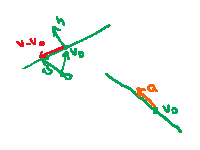
\includegraphics[height=4cm]{img/lecture26_drawing_1}
    \vspace{-110pt}
\end{wrapfigure}

Способы задания:
\begin{enumerate}
    \item $Ax + By = C \quad\quad (A, B) \neq (0, 0)$ --- нормаль.
    \item векторное уравнение $(v - v_0, n) = 0$, где $n$ --- нормаль.
    \item параметрическое уравнение $v = v_0 + at$, где $a$ --- направляющий вектор.

        \begin{math}
            \begin{cases}
                x = x_0 + a_1 t, \\
                y = y_0 + a_2 t.
            \end{cases} \quad
            \begin{gathered}
                a = (a_1, a_2) \\
                v_0 = (x_0, y_0)
            \end{gathered}
        \end{math}
\end{enumerate}

\paragraph{Уравнение прямой проходящей через две различные точки $(x_0, y_0)$ и $(x_1, y_1)$}

\begin{equation*}
    \begin{vmatrix} 
        x - x_0 & y - y_0 \\
        x_1 - x_0 & y_1 - y_0
    \end{vmatrix} = 0 \hspace{1cm}
    \frac{x - x_0}{x_1 - x_0} = \frac{y - y_0}{y_1 - y_0} \hspace{1cm}
    \begin{gathered}
        x_1 = x_0 \implies x = x_0, \\
        y_1 = y_0 \implies y = y_0.
    \end{gathered}
\end{equation*}


\subsection{Плоскости в $\RR^3$: различные способы задания, уравнение плоскости, проходящей через три точки, не лежащие на одной прямой}

\begin{wrapfigure}{r}{4.5cm}
    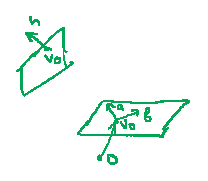
\includegraphics[width=4.5cm]{img/lecture26_drawing_2}
    \vspace{-30pt}
\end{wrapfigure}

Способы задания:

\begin{enumerate}
    \item $Ax + By + Cz = D \quad\quad(A, B, C) \neq (0, 0, 0)$ --- нормаль.
    \item векторное уравнение $(v - v_0, n) = 0$.
    \item параметрическое уравнение $v = v_0 + at + bs$, где $a, b$ --- направляющие векторы (базис в направляющем подпространстве).
\end{enumerate}

\paragraph{Уравнение плоскости, проходящей через 3 точки, не лежащие на одной прямой $(x_0, y_0, z_0), (x_1, y_1, z_1), (x_2, y_2, z_2)$}

\begin{equation*}
    \begin{vmatrix} 
        x - x_0 & y - y_0 & z - z_0 \\
        x_1 - x_0 & y_1 - y_0 & z_1 - z_0 \\
        x_2 - x_0 & y_2 - y_0 & z_2 - z_0
    \end{vmatrix} = 0
.\end{equation*}


\subsection{Прямые в $\RR^3$: различные способы задания, уравнение прямой, проходящей через две различные точки}

\begin{wrapfigure}{r}{3.5cm}
    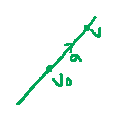
\includegraphics[width=2.5cm]{img/lecture26_drawing_3}
    \vspace{-30pt}
\end{wrapfigure}

Способы задания:
\begin{enumerate}
\item 
    \begin{math}
        \begin{cases}
            A_1 x + B_1 y + C_1 z = D_1, \\
            A_2 x + B_2 y + C_2 z = D_2
        \end{cases} \hspace{1cm} 
        \rk \begin{pmatrix} A_1 & B_1 & C_1 \\ A_2 & B_2 & C_2 \end{pmatrix} = 2
    \end{math}

\item векторное уравнение $[v - v_0, a] = 0$, где $v - v_0$ --- точка, $a$ --- направляющий вектор.
\item параметрическое уравнение $v = v_0 + at$. 

    \begin{math}
        \begin{gathered}
            v_0 = (x_0, y_0, z_0) \\
            a = (a_1, a_2, a_3)
        \end{gathered}
        \quad \longrightarrow \quad
        \begin{cases}
            x = x_0 + a_1 t, \\
            y = y_0 + a_2 t, \\
            z = z_0 + a_3 t.
        \end{cases}
        \quad \iff \quad
        \colorboxed{red}{\dfrac{x - x_0}{a_1} = \dfrac{y - y_0}{a_2} = \dfrac{z - z_0}{a_3}}
        \text{ --- каноническое уравнение прямой}
    \end{math}

    Если, например $a_1 = 0$, то пишут 
    \begin{math}
        \begin{cases}
            \displaystyle
            \frac{y - y_0}{a_2} = \frac{z - z_0}{a_3} \\
            x = x_0
        \end{cases}
    \end{math}
\end{enumerate}

\paragraph{Уравнение прямой, проходящей через $(x_0, y_0, z_0)$ и $(x_1, y_1, z_1)$}

\begin{equation*}
    \frac{x - x_0}{x_1 - x_0} = \frac{y - y_0}{y_1 - y_0} = \frac{z - z_0}{z_1 - z_0}
.\end{equation*}


\subsection{Взаимное расположение двух плоскостей, двух прямых, прямой и плоскости}

\subsubsection{Двух плоскостей}

\begin{wrapfigure}{r}{10cm}
    \vspace{-70pt}
    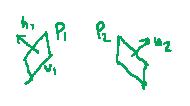
\includegraphics[width=5cm]{img/lecture26_drawing_4}
\end{wrapfigure}

\begin{enumerate}[nosep]
    \item \label{lec26:l1} Совпадают.
    \item \label{lec26:l2} Параллельны.
    \item Пересекаются по прямой.
\end{enumerate}

\medskip
$\hyperref[lec26:l1]{1)}, \ \hyperref[lec26:l2]{2)} \iff [u_1, u_2] = \overrightarrow{0}$.


\subsubsection{Двух прямых}

\begin{wrapfigure}{r}{10cm}
    \vspace{-70pt}
    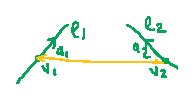
\includegraphics[width=5cm]{img/lecture26_drawing_5}
\end{wrapfigure}

\begin{enumerate}[nosep]
    \item \label{lec26:l3} Совпадают.
    \item \label{lec26:l4} Параллельны.
    \item \label{lec26:l5} Пересекаются в точке.
    \item Скрещиваются.
\end{enumerate}

\medskip
$\hyperref[lec26:l3]{1)}, \ \hyperref[lec26:l4]{2)} \iff [a_1, a_2] = \overrightarrow{0}$.

$\hyperref[lec26:l3]{1)}, \ \hyperref[lec26:l4]{2)}, \ \hyperref[lec26:l5]{3)} \iff (a_1, a_2, v_1 - v_2) = 0$.


\subsubsection{Прямой и плоскости}

\begin{wrapfigure}{r}{10cm}
    \vspace{-20pt}
    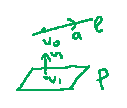
\includegraphics[height=2cm]{img/lecture26_drawing_6}
    \vspace{-110pt}
\end{wrapfigure}

Пусть $l$ --- прямая, $P$ --- плоскость.

\begin{enumerate}[nosep]
    \item \label{lec26:l6} $l \subseteq P$.
    \item \label{lec26:l7} $l \parallel P$.
    \item Пересекаются в точке.
\end{enumerate}

\medskip
$\hyperref[lec26:l6]{1)}, \ \hyperref[lec26:l7]{2)} \iff (a, n) = 0$.
